\section{Example 1: Safety}

Safety can be briefly characterized as the confidence that a software or technical system will not harm humans or cause major damage or financial loss. Airplanes or cars need to ensure functional safety according to ISE 61 508 or ISO 26262. An autonomous driving system must ensure that the intelligent breaks will not cause accidents.

\begin{figure}[t]
    \centering
    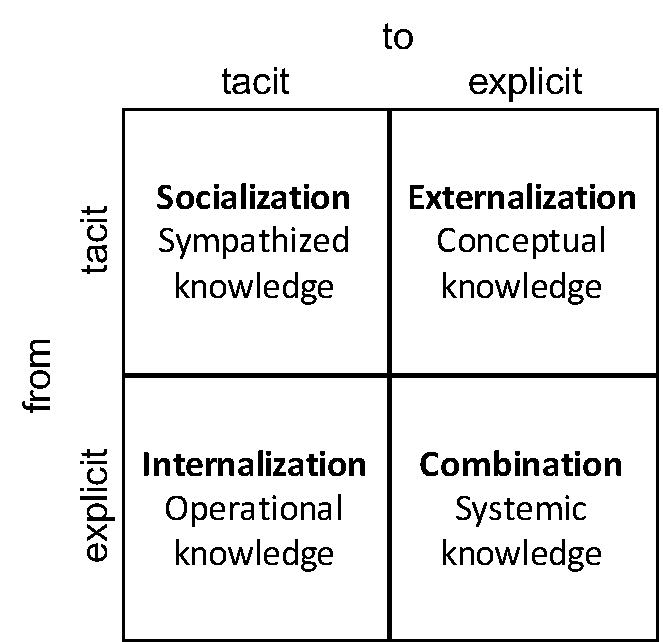
\includegraphics[width=0.5\columnwidth]{figs/nonaka95}
    \caption{Conversions between tacit and explicit knowledge \cite{Nonaka1995}.}
    \label{fig:nonaka1995}
\end{figure}

In our project on Requirements Engineering for large-scale agile system development \cite{Kasauli2017a}, many case companies develop safety critical systems and are subjected to regulation. 
These companies struggle to establish an effective approach to manage safety that still supports agile, incremental work. 
Regulations often require comprehensive tracing information that relates different system engineering artifacts to each other and allows to show how safety was systematically build into the system.
Further, %verifying the safety of large-scale systems takes significant resources and time.
%In 
in order to support incremental, agile development, it is desirable to also allow for incremental verification. 
For this and other reasons, safety must already be considered during creating the system architecture, e.g. by defining independent components, separating safety concerns from others, and provide redundancies for critical components.
This requires long term system knowledge, mainly created through \emph{combination} (Fig. \ref{fig:nonaka1995}) of existing system artifacts.

Yet, there is always a risk to include a change %to the system 
that effectively declines the safety of a component.
This risk must be mitigated just-in-time, for example by doing a change-impact-analysis to understand which components will be affected and then \emph{internalize} the existing knowledge about the system under construction.
Such existing knowledge is usually provided by existing engineering artifacts (in agile: code and its tests).
When a cross-functional team starts the development of a new feature for a safety critical system, one of the first steps is to do a hazard analysis. 
The result will inform the team about the safety criticality of the feature, which in turn defines the engineering method to be applied. 
In our experience, practitioners often reach out to domain experts to help them assess the system requirements efficiently, leading to emergent collaboration.
This activity can be considered to be just-in-time and relies on \emph{internalization} of existing system knowledge as well as on \emph{socialization} to discuss how the feature will affect functional safety.% of users and other stakeholders. 

The foundation for such reasoning is long-term knowledge about the desired (or required) level of safety. 
While this knowledge might have been established at one time face-to-face through socialization of domain experts, it is long-lasting and reusable (i.e. the next product will relate to very similar safety concerns). 
Thus, an efficient way of \emph{externalization} of this knowledge is required. 

Today, this externalization is not emphasized in many agile system development approaches.
Due to the long-lasting nature of safety considerations of systems, existing documentation can be reused after a company has transitioned from v-model or waterfall approaches to agile. 
However, we argue that updating and maintaining this knowledge must be considered in any approach to agile system development.